\documentclass[fleqn,11pt]{olplainarticle}
% Use option lineno for line numbers 
\usepackage{graphicx} 
\usepackage{float} 
\usepackage{subfigure} 
\title{Pairwise Relationships Prediction System}


\author{Hanzhong Wang\thanks{1029740}}
\author{Xinnan SHEN\thanks{1051380}}
\author{Ziyue WANG\thanks{1014037}}
\affil{Team Name: group8}
\affil{School of Computing and Information Systems, University of Melbourne}

\affil[]{\textit{\{hanzhongw,xinnan.shen, ziyue2\}}@student.unimelb.edu.au}


% \keywords{Keyword1, Keyword2, Keyword3}

% \begin{abstract}
% Please provide an abstract of no more than 300 words. Your abstract should explain the main contributions of your article, and should not contain any material that is not included in the main text. 
% \end{abstract}

\begin{document}
\maketitle
\flushbottom
\thispagestyle{plain}
\pagestyle{plain}


\section{Introduction}\label{intro}

\subsection{Background}\label{bgd}
\paragraph*{}
Nowadays, pairwise relationships are used to store many forms of data. However, when we build the pairwise relationships, it is inevitable that some edges between nodes are absent in the graph, which might mislead others a lot. Therefore, finding a way to predict the edges between nodes is an important step. In this project, we have implemented a system to predict the pairwise relationships between nodes by using machine learning tools. Given the nodes and some edges in the graph, the system can predict whether there is a relationship between them.  The results have shown that the machine learning model works well in predicting the edges between nodes. Although there are some errors, the model still have great performance.

\subsection{Related Works}\label{relaw}
\paragraph*{}
Many researches related to pairwise link prediction have been conducted. For example, Liben-Nowell has created a relationship prediction model that can be used in social networks \citep{liben2007link}. Also, Zhou et al. have mentioned that they have adopted machine learning tools to predict the relationships between people \citep{lu2011link}. In our project, we will also use machine learning methods to make predictions. Meanwhile, some researchers believe that deep learning is a strong tool that can be used to predict relationships \citep{wang2019}, which has also been adopted in our model.
% \paragraph*{}
% In this paper, the system implementation details will be deeply discussed. In section \ref{datafeature}, we will discuss the method of extract training data from given dataset and the process of feature engineering. In section \ref{appres}, the approaches we have used to design the system and their corresponding results will be mentioned. In addition, section \ref{analysis} will analyse the possible error in this system and the causes of these errors. Finally, section \ref{conclu} will make a conclusion and state the possible improvements of this system.



\section{Data Sampling and Feature Engineering}\label{datafeature}

\subsection{Data Sampling}\label{data}
\paragraph*{}
The original training data “train.txt” contains 20,000 records of user-follow from Twitter, with a total of 4,867,136 nodes(users). Due to oversized experimental data, in this experiment, we only randomly selected 50,000 edges (source node, target node) from the original data as the true edges (positive sample) of the experimental training data, and randomly selected 50,000 edges (source node, target node)  that do not exist in the original training data as the false edges (negative sample) of the experimental training data. 

\subsection{Feature Engineering}\label{feature}
\paragraph*{}
We first created an undirected graph using all of the given data and then generated multiple features of train data and test data based on the graph: resource allocation Index, Jaccard coefficient, and Adamic-Adar index, and preferential attachment score. In addition, according to the follower-followee relationship of the data nodes, we built a directed graph in which the source node points to the sink node. We predicted that if user M follows A, B, and C, and N is very similar to A, B, and C, we assume M may follow N. Thus, we generate two features based on the directed graph: cosine similarity and Jaccard similarity coefficient of the sink node and sinks list of the source node, which will help increase the accuracy of prediction.


\section{Approaches and Results}\label{appres}
% \paragraph*{}
% After we sampled data from the entire dataset and conducted feature engineering, we tried to use different kinds of machine learning tools to generate the results, including logistic regression, K-Nearest Neighbour and deep learning.

\subsection{Logistic Regression}\label{lr}
\paragraph*{}
Logistic Regression is suitable for binary classification problem, which we have treated as a baseline for this system \citep{menard_lr}. We have divided the processed data into training set and validation test \citep{scikit-learn}. To prevent the model from overfitting, we have used validation set not only to tune hyperparameters, but also to see the performance of the model in a very different dataset. Based on the performance of the model in the validation set, we have chosen the hyperparameters with the greatest accuracy to train the data and make predictions. The performance of Logistic Regression model can be seen as follows:

% table
\begin{table}[!htbp]
\centering
\caption{Logistic Regression Result}\label{tab:lr}
\begin{tabular}{ccc}
\toprule
Precision& Recall& F-1 Score\\
\midrule
0.99& 0.26& 0.41\\
\bottomrule
\end{tabular}
\end{table}
\paragraph*{}
From table \ref{tab:lr}, we can see that the logistic regression does not have a very good performance, but it is suitable to act as a baseline for this system.

\subsection{K-Nearest Neighbour}\label{knn}
\paragraph*{}
We have also used KNN classifier to try to improve the performance of the model \citep{Rebala2019}. Similar to what we have done in Logistic Regression, we have also divided the data into training set and validation set. By using scikit-learn tools \citep{scikit-learn}, we can train the model and predict the results more easily. Table \ref{tab:knn} has shown the results of K-Nearest Neighbour model. It is evident that KNN performs a little bit better than Logistic Regression, as the F-1 score is much higher. However, we still need to use some more powerful models to enhance the performance even further.

% table
\begin{table}[!htbp]
\centering
\caption{KNN Result}\label{tab:knn}
\begin{tabular}{ccc}
\toprule
Precision& Recall& F-1 Score\\
\midrule
0.62& 0.64& 0.63\\
\bottomrule
\end{tabular}
\end{table}



\subsection{Deep Learning}\label{dnn}
\paragraph*{}
In this project, we have also used deep learning to generate predictions. We have tried to use fully connected neural networks, and the activation function of output layer is sigmoid. The loss function is binary cross-entropy, which is suitable for binary classification problem \citep{tensorflow2015-whitepaper}. In particular, we have used the validation dataset to tune hyper-parameters so that we can select the model with the best performance to predict the final results.
\paragraph*{}
For DNN, we have tried models with 2, 3 and 4 hidden layers. The results is shown in figure \ref{fig:res}. From the graph, we can see that the performance of DNN has improved a lot, much better than Logistic Regression and KNN. In addition, the model with 2 hidden layers has the greatest F1-score in the validation set (82\%). Therefore, it performs best among all the models, and we have chosen this model to produce the final predictions.
\begin{figure}[H]
	\centering
	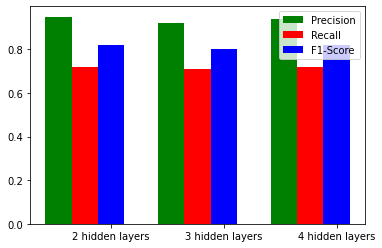
\includegraphics[scale=0.3]{result.png}
	\caption{Deep Neural Networks Result}
	\label{fig:res}
\end{figure}


\section{Critical Analysis}\label{analysis}
\paragraph*{}
The factors resulting in incorrect predictions include the problems within dataset and improper feature input. The problems within dataset are mainly due to the fact that the dataset is too large and the sink list of each source from the training set is not balanced. In order to solve this issue, we have sampled and analyzed the data from training set, and processed the training set into positive data and negative data. However, there are still some limitations. First of all, the accuracy of the positive data prediction greatly depends on the sampling data, which loses the information of the remaining data. Secondly, the method of generating negative data is to randomly choose the source node in the training set and the node in the sink list that does not exist in this source node as the new sink, which might lead to improper data selection. Finally, due to improper data selection, our model may have overfitting problems, which will affect the accuracy of prediction results.
\paragraph*{}
Logistic regression is a binary classification method. Compared with the naive Bayes method, logistic regression does not need to consider whether the features are related. Compared with decision tree and SVM, we can easily use the generated data to update the model by using online gradient descent. However, the dataset is too large and the generated feature space is very large in this project, which results in poor performance of logistic regression. The model is likely to suffer from underfitting problem and cannot handle a large number of multi-type features or variables well.
\paragraph*{}
In this project,  the performance of the KNN model is not very good, as this training set is large and each samples are not balanced. For example, some source nodes have very few nodes in the sink list, while others have quite many nodes in sink list, which results in imbalance distribution of data samples and a relatively large deviation. We have achieved better accuracy by using deep neural network compared with the above two methods. Because this method performs better than LR and KNN in feature space. By using deep neural network, we try to reduce the complexity of the neural network and focus on training the model with positive and negative characteristics generated by data sampling. Parameters such as the number of hidden layers can be adjusted to better capture the nature of input features and avoid overfitting. 


\section{Conclusion and Future Directions}\label{conclu}
\subsection{Conclusion}\label{con}
\paragraph*{}
Pairwise relationship is a useful relationship to store a number of data in real life. In this project, we have implemented a system to predict pairwise relationships, and the system can predict satisfactory results.
\subsection{Future Directions}\label{future}
\paragraph*{}
Although the system can generate satisfactory results, with high F1 score, its performance can be further improved by considering some other aspects. Firstly, feature engineering. It is worth trying to generate more complex features from the training data. Secondly, it is also a good idea to consider Convolutional Neural Networks, as it might have better performance. Finally, other ML tools might help. We could try some other machine learning methods, like SVM.



\bibliography{sample}
% \printbibliograpy
% \small{*All contributions were made by all teammates equally in a comprehensive manner, and therefore it is hard to distinguish specific responsibilities}
\end{document}
